% !TEX root = ../main.tex
\chapter{Le Web sémantique}
\label{annexe:semantic-web}
% TOOD: les ordinateurs et les utilisateurs VS
% ordinateurs et utilisateurs.

% the original text: ``The Semantic Web is an extension of the current
% web in which information is given well-defined meaning, better
% enabling computers and people to work in cooperation.''

L'expression \emph{``Web sémantique''} trouve ces origines dans un
article révolutionnaire publié par Tim Berners-Lee \emph{et
  al.}~\cite{berners2001semantic} en \date{2001}. Le terme fait
d'abord référence à la vision du Web de demain comme un vaste espace
d'échange de ressources entre les êtres humains et les machines
permettant une exploitation, qualitativement supérieure, de grands
volumes d'informations et de services variés. D'après ses promoteurs
\emph{``le Web sémantique est une extension du Web actuel avec une
  signification bien définie des informations. Il permet une meilleur
  coopération et d'échanger l'information entre les ordinateurs et les
  utilisateurs.''}\medskip

Aujourd'hui, le Web Sémantique désigne une infrastructure
technologique visant à rendre le contenu des ressources du Web
accessible et utilisable par des logiciels ou des agents grâce à un
ensemble des langages et des standards initiés et maintenus par le
consortium \acrshort{w3c}. Ces langages sont organisés en couches
d'expressivité croissante permettant l'ajout d'une
\emph{\textbf{``sémantique explicite''}} au contenu des ressources
Web. Cette vision va transforme le Web actuel de documents en Web des
connaissances (ou \emph{Knowledgeable web}~\cite{decker2000semantic}),
ce qui contribue largement au développement de nouvelles approches
plus flexibles pour le partage des données, la réutilisation et
l'intégration de différentes applications.\medskip

%% TODO: éliminer la duplication du terme "Web sémantique"
Dans la suite, nous introduisons la vision globale du Web sémantique,
leur objectifs et principes
fondamentaux~\ref{sec:semantic-web-vision}. Ensuite Nous allons
présenter les principaux standards et langages développés par la
communauté pour la réalisation et la concrétisation du web
sémantique~(\ref{sec:semantic-web-rdf}~\ref{sec:semantic-web-owl}).

\newpage
\section{La vision du Web sémantique}
\label{sec:semantic-web-vision}

%!TEX root = ../../main.tex
\begin{figure}[h]
    \centering
    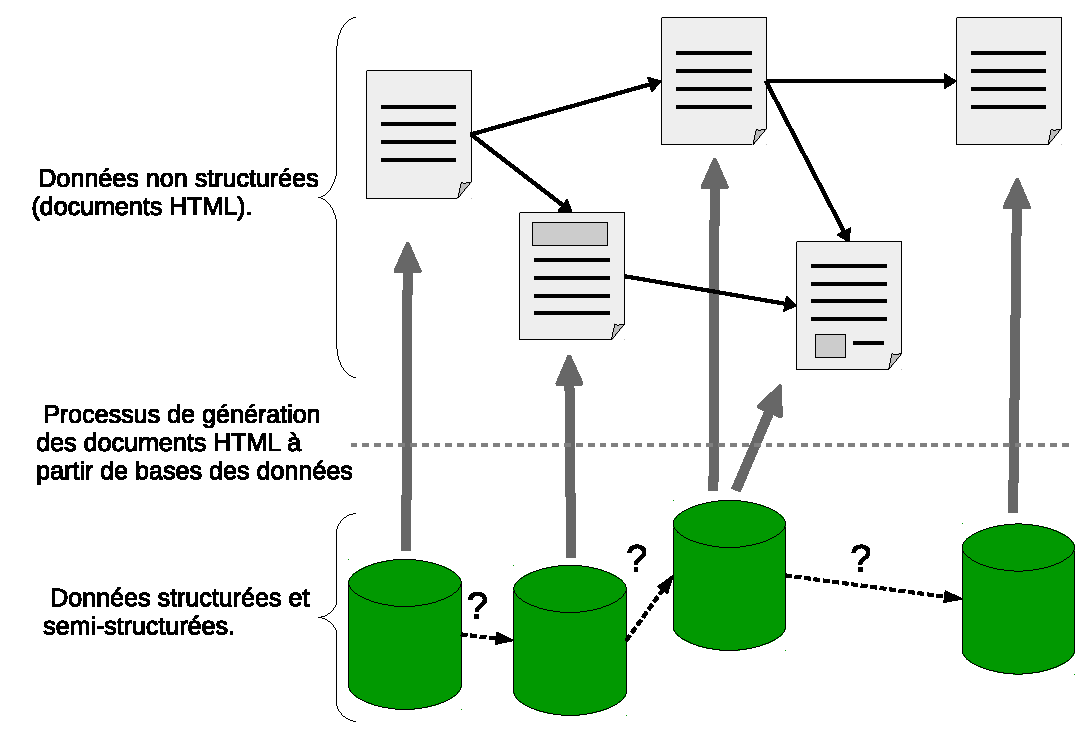
\includegraphics[width=1\textwidth]{figs/A/structured-and-unstructured-data-on-the-web.eps}
    \caption{Les données structurés et non-structurés du
      Web~\cite{antoniou2012semantic}.}\label{fig:structured-and-unstructured-data-on-the-web}
\end{figure}
%%% Local Variables:
%%% mode: latex
%%% TeX-master: "../../main"
%%% End:


% des phrases trop longues !!
Le Web actuel est essentiellement \emph{\textbf{syntaxique}}, dans le
sens que la structure des documents est bien définie mais que son
contenu reste quasi inaccessible aux traitements machines. Il s'agit
d'un Web de documents, les ressources sont structurées en
\acrshort{html} et identifiés de manière unique par des \acrshort{uri}
reliés entre eux par des liens \emph{hypertextes}. L'information est
essentiellement textuelle et la structure riche qui est généralement
conçus au préalable dans des schémas relationnelles est presque
complètement perdu dans le processus de publication de telles données
sous formes des documents \acrshort{html} (ce qui illustré dans la
figure~\ref{fig:structured-and-unstructured-data-on-the-web}).\medskip

La nouvelle génération de Web nommée \emph{``Le Web sémantique''} a
pour ambition de lever cette difficulté. Les ressources du Web seront
plus aisément accessibles aussi bien par l'homme que par la machine,
grâce à la représentation \emph{\textbf{sémantique}} de leurs
contenus. La suite de cette section a pour but de expliquer les
principes fondamentaux et les idées principales derrière le Web
sémantique~\ref{sec:semantic-web-design-decisions}, ainsi que le socle
technologique permettant la concrétisation de ces
idées~\ref{sec:semantic-web-stack}.\medskip

\subsection{Principes fondamentaux du Web sémantique}
\label{sec:semantic-web-design-decisions}

Le Web sémantique, ou le Web de données (dans son vision
futuriste~\cite{bizer2008linked}) suit différents principes de
conception, qui peuvent être résumés comme
suit~\cite{antoniou2012semantic}:\medskip

\begin{enumerate}
\item Rendre les données structurées et semi-structurées (illustré
  dans la
  figure~\ref{fig:structured-and-unstructured-data-on-the-web})
  disponibles dans formats normalisés et standardisés sur le
  Web;\medskip

\item Rendre non seulement les ensembles de données, mais aussi les
  éléments individuels de données et leurs relations implicites
  accessibles sur le Web;\medskip

\item Décrire la sémantique de ces données dans un formalisme bien
  définie, afin que cette sémantique peuvent être accessibles et
  traitables par des machines.
\end{enumerate}

Ces décisions conceptuelles sont la résultat directe d'un aperçu
principal qui nous amène à un grand progrès vers la vision du Web
sémantique. En effet, l'idée générale est de publier et interconnecter
l'structure sous-jacente de l'ensemble de données au lieu de
simplement publier et interconnecter des pages
\acrshort{html}.\medskip

Un aspect clé du Web est le fait que son contenu est totalement
distribué~\cite{berners1989information}, cette caractéristique
fondamentale contribue énormément à la naissance et la propagation de
Web tel que nous le connaissons aujourd'hui. En effet, la vision du
Web sémantique doit prendre en compte de la nécessaire ouverture du
Web et son architecture décentralisée, cette rétrocompatibilité
manifeste dans la traduction des trois principes mentionnées
précédemment sous forme d'un ensemble de décisions techniques
~\cite{antoniou2012semantic}:\medskip

\begin{enumerate}
\item Utiliser un graphe étiqueté comme un modèle de données pour
  représenter les ressources Web et ses relations. Le standard
  \acrshort{rdf} (parfois nommé un langage) est utilisé comme un
  formalisme pour représenter ces graphes;\medskip

\item Utiliser \acrshort{uri} pur identifier les éléments de données
  individuels et ses relations qui apparaissent dans la structure de
  données sous-jacente. Encore une fois, cela se reflète dans la
  conception du \acrshort{rdf}.;\medskip

\item Utiliser des ontologies (vocabulaires hiérarchiques de types et
  de relations) pour représenter formellement la sémantique prévues
  des données. Des formalismes tels que \acrshort{rdfs} et
  \acrshort{owl} sont utilisés pour ce effet.
\end{enumerate}\bigskip

\newpage
\subsection{Technologies clés du Web sémantique}
\label{sec:semantic-web-stack}

Pour la mise en place d'un Web sémantique, un ensemble des étapes
doivent être considérées pour l'implémentation des principes
ci-dessus~\ref{sec:semantic-web-design-decisions}. Premièrement, il
faut un \textbf{syntaxe standard} pour représenter les données et les
\emph{méta-données}. Deuxièmement, Avoir un accord suffisant sur un
\textbf{vocabulaire} pour les \emph{méta-données} afin de partager la
sémantique prévues des données. Enfin, publier un grand volume de
données dans les formats de la première étape en utilisant les
vocabulaires de la deuxième étape~\cite{antoniou2012semantic}.\medskip

%!TEX root = ../../main.tex
\begin{figure}[h]
    \centering
    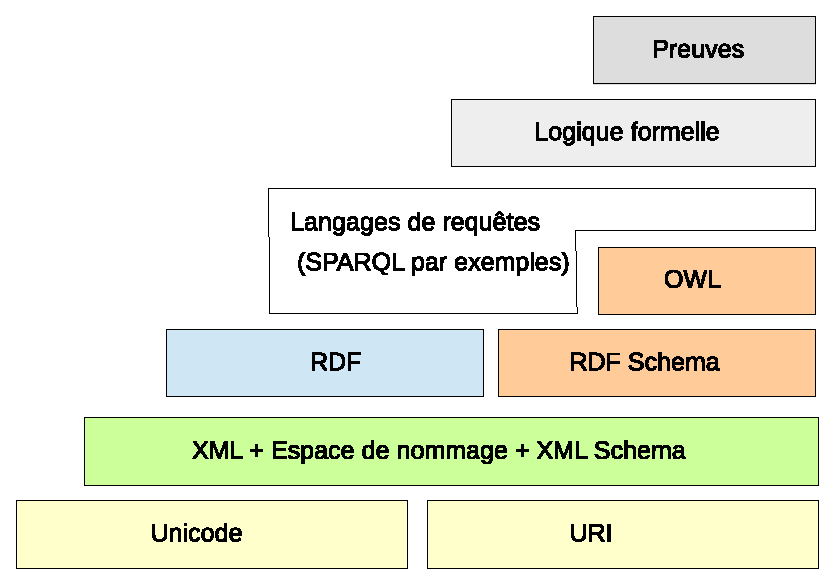
\includegraphics[width=0.85\textwidth]{figs/A/semantic-web-stack.eps}
    \caption{La pyramide du Web sémantique.}\label{fig:semantic-web-stack}
\end{figure}
%%% Local Variables:
%%% mode: latex
%%% TeX-master: "../../main"
%%% End:


Au cours de les deux dernières décennies, des progrès substantiels ont
été réalisés dans chacun de ces trois étapes. Des langages comme
\acrshort{rdf}, \acrshort{rdfs} et \acrshort{owl} (organisés en
couches d'expressivité croissante) ont reçu l'appui officiel du
consortium \acrshort{w3c}. Cet ensemble de \emph{``couches''} est
appelé, par ce dernière, \emph{``la pyramide des langages du Web
  sémantique''} (illustrée dans la
figure~\ref{fig:semantic-web-stack}). Plusieurs milliers de
vocabulaires ont été publiés dans ces formats (vocabulaire
schema.org~\footnote{\url{http://schema.org/}}, par exemple), ainsi
que le développement rapide du \emph{Linked
  Data}~\footnote{\url{http://linkeddata.org/}} a donné lieu à de
nombreux milliards d'objets et leurs relations deviennent disponibles
sur le Web s'appuyant sur une syntaxe et des vocabulaires communes.

Deux types de bénéfices sont motivés par cette organisation en couches
des langages du Web sémantique illustrée dans
figure~\ref{fig:semantic-web-stack}:\medskip

\SpecialItem
\begin{itemize}
\item Elle doit permettre de choisir le langage d’expressivité et de
  complexité adapté aux besoins d'une modélisation à réaliser;\medskip

\item Elle permet une approche graduelle dans les processus de
  standardisation de ces langages naissants (\acrshort{owl} n'a vu
  le jour qu'en \date{2001}~\cite{fensel2001oil} et est une
  recommendation du \acrshort{w3c} depuis seulement
  \date{2004}~\cite{mcguinness2004owl}).\medskip
\end{itemize}
\enddescription

Dans la construction d'une couche du Web sémantique sur le dessus de
l'autre, deux principes doivent suivie~\cite{antoniou2012semantic}:

\renewcommand{\descriptionlabel}[1]{\hspace{0.5cm}\textbullet~\textsf{#1}}
\begin{description}
\item[Compatibilité descendante]: Les agents logiciels spécialisés
  d'une couche devraient également être en mesure d'utiliser et
  interpréter l'information écrite à des niveaux inférieurs de
  pyramide. Par exemple, les agents qui peuvent accéder à la
  sémantique de \acrshort{owl} peuvent profiter pleinement des
  informations exprimées en \acrshort{rdf} et \acrshort{rdfs};

\item[Compatibilité ascendante partielle ]: Les gents logiciels
  spécialisés d'une couche devrait être en mesure de profiter au moins
  \textsf{partiellement} de l'information aux niveaux plus élevés. Par
  exemple, un agent spécialisé seulement à l'analyse syntaxique des
  documents \acrshort{rdf} et \acrshort{rdfs} pourraient interpréter
  une connaissance exprimée en \acrshort{owl} partiellement.
\end{description}
\enddescription

La figure~\ref{fig:semantic-web-stack} montre \emph{``la pyramide du
  Web sémantique''} qui décrit les couches principales de la
conception du Web sémantique. Cette vision est proposée initialement
par Tim Berners-Lee~\cite{berners2000xml} en \date{2000} au sien de
\acrshort{w3c}.\medskip

Le bas de la pyramide correspond aux technologies rassemblées sous le
nom du web de documents et qui permettre de fournir les bases du Web
sémantique. Nous trouvons à dans ce niveau là, l'dentificateur de
ressource internationalisé~\acrshort{uri}~\footnote{Il faut bien noter
  la différence entre les spécifications URL, URL et URN expliquée
  dans ce lien \url{http://www.w3.org/TR/uri-clarification/}.} qui
permet d'attribuer un \emph{identifiant unique} à un ensemble de
ressources sur le Web (documents, numéros téléphone, numéros
\acrshort{isbn}, etc), ainsi que le standard
\textsf{Unicode}~\footnote{\url{http://unicode.org/}.}  pour le codage
de textes dans différentes langues.\medskip

\acrshort{xml}~\cite{bray1998extensible} est un composant fondamental
qui assure \emph{l'interopérabilité
  syntaxique}~\cite{decker2000semantic} de cette infrastructure, il
fournit un mécanisme simple et puissant pour représenter des données
échangeables sur le Web. Le langage
\acrshort{xmls}~\cite{fallside2004xml} permet de construire des
documents \acrshort{xml} suivant un syntaxe et une structure
hiérarchique spécifique et les étendre avec des types de
données.\medskip

\acrshort{rdf}~\cite{lassila1999resource} est le modèle de données
fondamental pour le Web sémantique, il permet d'une meilleure
représentation et exploitation des \emph{méta-données} structurées et
fournit un support pour \emph{l'interopérabilité
  sémantique}~\cite{decker2000semantic}. \acrshort{rdfs}~\cite{brickley2000resource}
est un langage qui sert á définir un vocabulaire pour décrire les
propriétés et les classes des ressources \acrshort{rdf} et fixer une
\emph{sémantique} partagée des ressources Web.\medskip

\acrshort{rdfs} peut être considéré comme un langage primitive pour la
représentation des connaissances et de définir des
ontologies~\cite{antoniou2012semantic}. \acrshort{owl}~\cite{martin2004owl}
ajoute plus de vocabulaire pour décrire les propriétés et les classes,
les relations entre les classes, cardinalité, égalité, typage de
propriétés plus riche, caractéristiques des propriétés et les
hiérarchies des propriétés et des classes.\medskip

Les couches supérieures de l'architecture de Web sémantique
contiennent la couche logique qui permet de l'écriture des règles
logiques de raisonnement et d'inférence et la couche de preuve qui
exécute et évalue ces règles utilisées.

\section{La description des ressources Web: RDF(S)}
\label{sec:semantic-web-rdf}

%TODO: vérifier surtout la dernière phrase entres les parenthèses.
\acrshort{rdf} fournit un modèle de données flexible et indépendant de
tout domaine pour représenter les données et \emph{méta-données}
sous-jacentes du Web~\cite{decker2000semantic}, son composant de base
est le triplet \emph{``suject-propriété-object''}, appelé une assertion
ou encore une déclaration (\emph{``Statement''} en Anglais), c'est
pourquoi il est mentionné parfois comme un langage assertionnel. Il
faut bien noter la standard \acrshort{rdf} n'exige aucun format
particulier pour la sérialisation (et que \acrshort{xml} est juste un
autre).\medskip

%% TODO: Why use RDF?

\newpage
Puisque le \acrshort{rdf} est pas lié à un domaine particulier, il est
nécessaire pour un utilisateur de définir \emph{une terminologie}
qu'ils utilisent au sein de ces déclarations. Le langage
\acrshort{rdfs} permet aux utilisateurs de définir précisément comment
leur vocabulaire (leur terminologie) doit être interprétée, c'est
l'habileté de attribuer une \emph{\textbf{sémantique explicite}} à un
ensemble de données (ressources Web).\medskip

Pour résumer, \acrshort{xml} peut être vu comme la couche de
sérialisation syntaxique, \acrshort{rdf} comme un modèle de
base. \acrshort{rdfs} offre des primitives de représentation de
connaissances structurées en \acrshort{rdf} et l'ajoute une sémantique
prévue.\medskip

Dans cette section, nous présentons le standard \acrshort{rdf}
~\ref{sec:semantic-web-rdf-rdf}, ainsi que ses syntaxes courantes pour
le sérialiser. Ensuite, Les bases de langage \acrshort{rdfs} et ses
composantes principales sont introduites
en~\ref{sec:semantic-web-rdf-rdf}.\medskip

\subsection{RDF~: Le modèle de données}
\label{sec:semantic-web-rdf-rdf}

les concepts fondamentaux de \acrshort{rdf} sont les ressources, les
propriétés, les assertions (déclaration) et les graphes.

\subsubsection{Ressources}
\label{sec:semantic-web-rdf-rdf-resources}

Une ressource est un élément constitutif de base de l'architecture du
Web, elle désigne un entité qui peut être référencé par une
\acrshort{uri}. Cela veut dire qu'une ressource peut être une page Web
mais pas nécessairement, il peut désigne également un élément nom
présent physiquement sur le Web comme un livre imprimé, qui sera alors
référencé par exemple par son numéro \acrshort{isbn}.

\subsubsection{Propriétés}
\label{sec:semantic-web-rdf-rdf-properties}

Les propriétés sont des ressources qui décrivent les relations entres
des autres ressources, par exemple \emph{``écrit par''} et \emph{``est
  de type de''}. Comme toutes les ressources, les propriétés sont
identifiées par des \acrshort{uri}, une propriété peut être aussi
\emph{déréférencée} pour trouver une description textuelle de cette
propriété.

\subsubsection{Assertions}
\label{sec:semantic-web-rdf-rdf-statements}
La structure fondamentale en \acrshort{rdf} est un triplet, composé
d'un sujet, une propriété et un objet. Un triplet s'interprète comme
suit: \emph{``le sujet a pour propriété l'objet''}.
%% TODO: citer un exemple

\subsubsection{Graphes}
\label{sec:sec:semantic-web-rdf-rdf-graphs}

% \renewcommand{\lstlistingname}{Document}
% \lstinputlisting[language={XML},caption={Example d'un RDF/XML
%   document}]{appendices/example.rdf}~\label{doc:rdf/xml}

\subsection{RDFS~: L'ajout de sémantique}
\label{sec:semantic-web-rdfs}

\section{Langage de définition des ontologies~: OWL}
\label{sec:semantic-web-owl}

% What is semantic web?

% Le Web tel que nous le connaissons aujourd'hui est encore conforme à
% la vision initiale.

% Le Web a été conçu principalement pour une utilisation par les
% humains. Néanmoins, il existe un effort visant à automatiser son
% utilisation et d'être plus accessible pour les machines.

% \cite{bartalos2011effective} The Web was primarily designed for use
% by humans. Nevertheless, there is an effort to automate its use and
% bring the Web more accessible for machines. This has brought forward
% the need for machine processable representations of semantically
% rich information. This has brought forward the need for machine
% processable representations of semantically rich information: a
% vision at the heart of the Semantic Web

% Dans un premier temps, on va essayer de clarifier la notion d'un
% service Web sémantique, puis étudier les langages émergeants qui
% permettent de décrire ce type de service Web.

% L'objectif premier du Web sémantique est de définir et lier les
% ressources du Web afin de simplifier leur utilisation, leur
% découverte, leur intégration et leur réutilisation dans le plus
% grand nombre d'applications \cite{berners2001semantic}. Le Web
% sémantique doit fournir l'accès à ces ressources par l'intermédiaire
% de descriptions sémantiques exploitables et compréhensibles par des
% machines. En effet, Les technologies du Web sémantique complètent le
% Web actuel avec des outils sémantiques. Il ne s'agit donc pas de
% créer un nouveau Web ou un Web séparé de l'existant : ce Web de
% données repose entièrement sur les technologies et concepts qui ont
% fait le succès du Web tel que nous le connaissons aujourd'hui
% \cite{bertails2010web}.

% La réalisation du Web sémantique trouve ces racines dans le
% développement des langages de balises inspiré par des travaux issus
% de la communauté AI \cite{mcilraith2001semantic}, tels que
% \textsc{OIL} \cite{fensel2001oil}, \textsc{DAML+OIL}
% \cite{horrocks2002daml+oil} et \textsc{DAML+OTN}
% \cite{mcguinness2003daml} (ces deux derniers langages font partie de
% la famille \acrshort{daml}).

% TODO refactor Ces langages ont une sémantique bien définies et
% permettent le balisage et la manipulation des taxonomies complexe et
% des relations logiques entre les entités sur le
% Web. \cite{fensel2000creating}

% \input{figs/3w_to_sws.tex}

% Cette description repose sur des ontologies. Selon Gruber
% \cite{gruber1993translation}, une ontologie est une spécification
% explicite d'une conceptualisation. Une conceptualisation est un
% modèle abstrait qui représente la manière dont les personnes
% conçoivent les choses réelles dans le monde et une spécification
% explicite signifie que les concepts et les relations d'un modèle
% abstrait reçoivent des noms et des définitions explicites. Le Web
% sémantique est devenu un domaine à part entière, preuve en est la
% création en 2001 du groupe de travail sur ce sujet par le
% \textsc{W3C}.

%%% Local Variables:
%%% mode: latex
%%% TeX-master: "../main"
%%% End:
